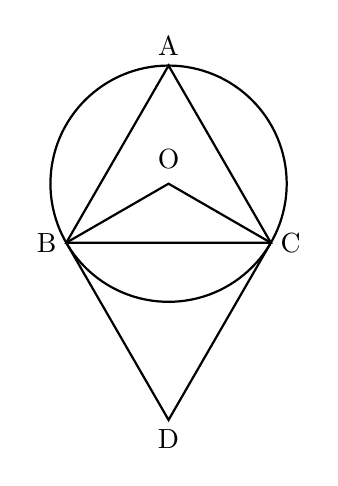
\begin{tikzpicture}[scale=1]

    % --- Coordinates ---
    % O is the center of the circle
    \coordinate (O) at (0,0);
    
    % Points on the circle (Radius 1.5cm)
    \coordinate (A) at (90:1.5);   % Top vertex
    \coordinate (B) at (210:1.5);  % Bottom-left vertex
    \coordinate (C) at (330:1.5);  % Bottom-right vertex
    
    % D is the external point where tangents from B and C meet
    % Calculated based on geometry: OD = radius / cos(angle/2)
    \coordinate (D) at (270:3);

    % --- Circle ---
    % Drawing the circumscribed circle centered at O
    \draw[thick] (O) circle (1.5);

    % --- Geometric Lines ---
    % 1. Triangle ABC inscribed in the circle
    \draw[thick] (A) -- (B) -- (C) -- cycle;
    
    % 2. Radii OB and OC forming triangle OBC
    \draw[thick] (B) -- (O) -- (C);
    
    % 3. Tangents BD and CD meeting at external point D
    \draw[thick] (B) -- (D) -- (C);

    % --- Point Labels ---
    % Positioned exactly as shown in Figure 19
    \node[above] at (A) {A};
    \node[left] at (B) {B};
    \node[right] at (C) {C};
    \node[above=2pt] at (O) {O};
    \node[below] at (D) {D};

\end{tikzpicture}